\chapter{pystl}
 pystl是處理stl檔案的python開源程式,無須打開CAD軟體即可編輯操作stl檔案,可以輕易使物體移動、轉動與縮放的動作。目前可以把輸入的ASCLL 或 binary STL檔案全部輸出成ASCLL STL。\\
 

\section{pySTL 功能}
\begin{itemize}
\item 打開text.stl檔案
\begin{lstlisting}[caption=\Large 輸入檔案]
import pySTL
model = pySTL.STLmodel('text.stl')

\end{lstlisting}
 
\item 物體向x軸移動10單位
 \begin{lstlisting}[caption=\Large 移動]
import numpy
movement = numpy.array([10, 0, 0])
model.translate(movement)

\end{lstlisting}

\item 物體質心移動到座標原點
 \begin{lstlisting}[caption=\Large 移動]
model.translate(-c)

\end{lstlisting}

\item 物體向X軸轉90度(角度是徑度)
 \begin{lstlisting}[caption=\Large 轉動]
R= pySTL.rotationAboutX(-3.14149/2)
model.rotate(R)

\end{lstlisting}

\item 物體縮小10%
 \begin{lstlisting}[caption=\Large 縮放]
scale = 0.1
model.scale(scale)

\end{lstlisting}


\item 質心顯示
 \begin{lstlisting}[caption=\Large 數值]
c = model.get_centroid()
print(c)

\end{lstlisting}

\item 體積顯示
 \begin{lstlisting}[caption=\Large 數值]
v = model.get_volume()
print(v)

\end{lstlisting}

\item 產生newText.stl檔案
\end{itemize}
 \begin{lstlisting}[caption=\Large 產生新stl檔案]
model.write_text_stl('newText.stl')
\end{lstlisting}

\section{為何要使用pySTL?}

由於預設場景裡CAD檔案與.STL的座標系是不相同,且.stl(mm)與coppeliasim(m) 的單位也不相同,所以當人們在不同軟體間操作,若是沒有注意到各個檔案的關係,會發生(如:圖5.1)物體方向錯誤或者尺寸錯誤,則必須要打開CAD軟體,使用軟體的移動、旋轉、縮放等工具把問題修正再轉成stl格式放進Coppeliasim場景,這一來一往所花費的時間是耗時的。\\

\begin{figure}[hbt!]
\begin{center}
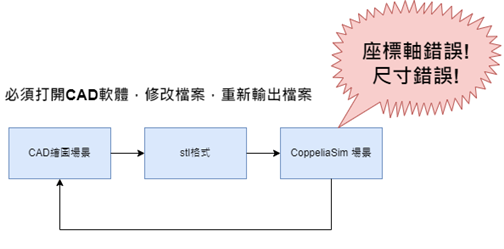
\includegraphics[scale=1]{正常轉檔流程}
\caption{\Large 正常轉檔流程}\label{正常轉檔流程}
\end{center}
\end{figure}

當檔案錯誤時,無須打開CAD軟體,只要編輯器啟動pySTL 代碼,輸入想要修改的參數按下執行,即可產生正確且最新版本的stl檔案,有了這項工具,即使電腦裡沒有繪圖軟體,也能立刻修改出正確的檔案,這將會是簡單又省時的操作來完成目標。(如:圖5.2)\\

\begin{figure}[hbt!]
\begin{center}
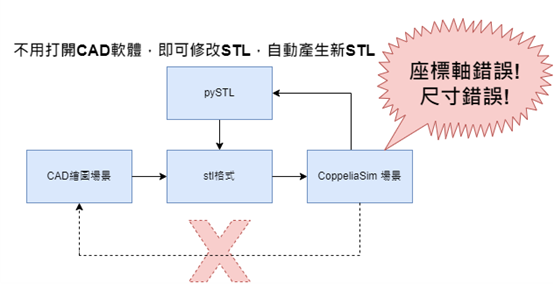
\includegraphics[scale=1]{pystl轉檔流程}
\caption{\Large pystl轉檔流程}\label{pystl轉檔流程}
\end{center}
\end{figure}

\section{如何使用pySTL?}
因為pySTL是一個開源套件,所以我們先在github 裡git clone pySTL整個資料夾下載出來。(如:圖5.3)
\begin{figure}[hbt!]
\begin{center}
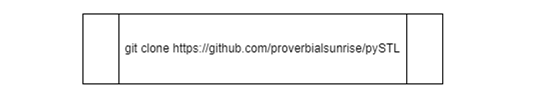
\includegraphics[scale=1]{clone pySTL}
\caption{\Large clone pySTL}\label{clone pySTL}
\end{center}
\end{figure}

這裡我們先當作檔案已經排除錯誤可以直接使用,因為資料裡的pySTL.py與sample.py有多處地方是錯誤的需要去解決,我們將詳細的解決步驟放到第8章節的問題討論裡。\\

\section{ pySTL操作設定}
首先打開sample.py檔案,輸入想要操作的名稱的STL檔。\\

 \begin{lstlisting}[caption=\Large 輸入名稱]
import pySTL
from numpy import array

#Load a model from a file.
model = pySTL.STLmodel('uArm_binary.stl')

\end{lstlisting}

在這裡我們選擇的檔案是uArm\_binary.stl檔案,並且可以先使用print,使我們可以先取得原本stl檔案的體積與質心數值。 \\

 \begin{lstlisting}[caption=\Large 數值]
v = model.get_volume()
print(v)

\end{lstlisting


\begin{figure}[hbt!]
\begin{center}
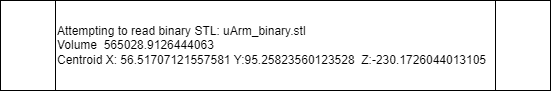
\includegraphics[scale=1]{ 體積與質心數值顯示}
\caption{\Large 體積與質心數值顯示}\label{ 體積與質心數值顯示}
\end{center}
\end{figure}

我們輸入pySTL.rotationAboutX(-3.14159/2),使物體能夠向x軸轉動90度,這裡需要注意的點是,角度的單位是徑度。\\

 \begin{lstlisting}[caption=\Large 向X軸轉90度]
#Rotate the model 90 degrees about the X-axis
R2 = pySTL.rotationAboutX(-3.14159/2)

model.rotate(R2)

c = model.get_centroid()
print ("Centroid1 " +  "X: " + str(c[0]) + " Y:" + str(c[1]) + "  Z:" + str(c[2]))

\end{lstlisting}

因為stl檔案的單位mm,但是coppeliasim模擬的場景的單位是m,所以我們必須使用scale=0.001,使物體縮小1000倍在使用model.write\_text\_stl來產生檔案。(如圖:圖5.3)\\

 \begin{lstlisting}[caption=\Large 縮小1000倍]
#Scale the model down by 1000%
scale = 0.001
model.scale(scale)

c = model.get_centroid()
print ("Centroid2 " +  "X: " + str(c[0]) + " Y:" + str(c[1]) + "  Z:" + str(c[2]))
model.write_text_stl('uArm_scale_down_0.001.stl')

\end{lstlisting}

最後我們把生成好的uArm\_scale\_down\_0.001stl放進coppeliasim場景裡面(圖5.4)我們可以發現uArm手臂的尺寸與方向都是正確的,無須再調整。\\

\begin{figure}[hbt!]
\begin{center}
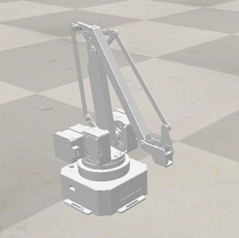
\includegraphics[scale=1]{uArm scale down coppeliasim}
\caption{\Large uArm scale down coppeliasim}\label{uArm scale down coppeliasim}
\end{center}
\end{figure}

\section{程式流程}

首先我們執行sample.py的啟動檔,導入pySTL模組,即可讀取STL檔案,得知物體體積與質心數值後,輸入想要的物體位置與比例縮放,來達成最終理想的STL檔案。(圖:5.5)\\

\begin{figure}[hbt!]
\begin{center}
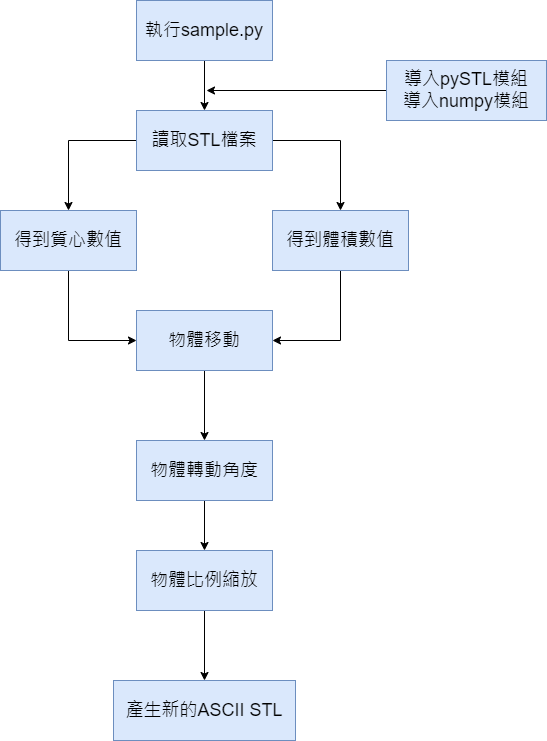
\includegraphics[scale=1]{sample.py程式流程}
\caption{\Large sample.py程式流程}\label{sample.py程式流程}
\end{center}
\end{figure}

\subsection{pySTL.py程式流程} 
(圖:5.6)我們讀取STL會先判斷各個種類的STL檔案,分別使用不同的方法去讀取檔案,當可以成功讀取檔案時,我們即可以使用ASCII的規格來寫入進去(solid	表面對法線	三維三角形頂點),即可產生ASCII STL檔案。\\

    我們使用每個三角形的頂點與原點形成一個四面體,計算每個模型體積用於得到三維形狀的質心(使用第6章的理論來求解),即可得用於物體的移動、轉動與縮放。\\

\begin{figure}[hbt!]
\begin{center}
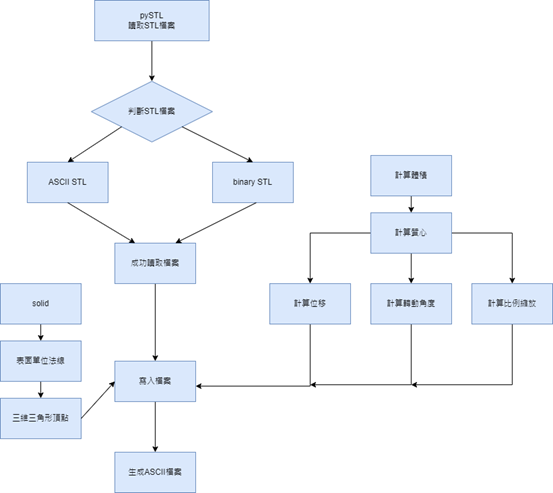
\includegraphics[scale=1]{pySTL.py程式流程}
\caption{\Large pySTL.py程式流程}\label{pySTL.py程式流程}
\end{center}
\end{figure}


